\chapter{3D Rekonstruktion}

\label{ch:eval-3d}

%----------------------------------------------------------------------------------------

\section{Wahl des Test-Objekts}

Zum Vergleichen der 3D-Rekonstruktions-Fähigkeiten verschiedener
Softwarelösungen haben wir uns ein geeignetes Objekt gesucht: Freistehend,
unregelmässig geformt und nicht ganz trivial rekonstruierbar. In der Nähe des
Bächlihofes in Jona wurden wir fündig: Dort stand ein grosser, für unsere Zwecke
gut geeigneter Stroh-Hase.

Wie auch im \autoref{workflow:hsr:drone} beschrieben, erfassten wir den Hasen
mit einem TBS Discovery Pro Quadrokopter und einer Sony Alpha 5100 Kamera. Für
dieses Dataset speicherten wir jedoch keine GPS-Daten, diese wären auf dieser
kleinen Fläche wohl nicht genügend genau.

Das resultierende Dataset enthält 315 Bilder, gesamthaft 3.1 GiB.

\begin{figure}[H]
	\centering
	\includegraphics[width=\textwidth]{images/rabbit4.jpg}
	\caption{Erfassung Bildmaterial Strohhase}
	\label{img:rabbit4}
\end{figure}

%----------------------------------------------------------------------------------------

\section{Resultate}

\subsection{Rekonstruktionsdauer}

Folgende Tabelle vergleicht die Rekonstruktionsdauer für die Sparse Cloud, die
Dense Cloud und – wo von der Software unterstützt – das Mesh.

\begin{figure}[H]
	\begin{tabularx}{\textwidth}[H]{Xccc}
		\toprule
		\textbf{Software} & \textbf{Sparse Cloud} & \textbf{Dense Cloud} & \textbf{Mesh} \\
		\midrule
		VisualSFM & 1h 13m & 1h 49m & n/a \\
		Pix4Dmapper Pro & 1h 40m & 3h 46m & 13m \\
		PhotoScan Pro & 3h 50m & 8h 11m & 8m \\
		\bottomrule
	\end{tabularx}
\end{figure}

\subsection{Komplexität der Resultate}

Als Vergleichsmass für die Komplexität der Resultate haben wir die Anzahl der
Punkte in der verdichteten Punktwolke sowie die Anzahl der Vertizes im Mesh
verwendet.

Dies ist natürlich nur bedingt aussagekräftig, da die Anzahl der Punkte bzw.
Vertizes von den Konversions-Parametern abhängig ist und auch nicht zwingend
etwas über die Qualität des Modells aussagt.

\begin{figure}[H]
	\begin{tabularx}{\textwidth}[H]{Xcc}
		\toprule
		\textbf{Software} & \textbf{Punkte in Punktwolke} & \textbf{Vertizes in Mesh} \\
		\midrule
		VisualSFM & 4'998'104 & n/a \\
		Pix4Dmapper Pro & 27'921'022 & 494'359 \\
		PhotoScan Pro & 11'823'773 & 397'244 \\
		\bottomrule
	\end{tabularx}
\end{figure}

%----------------------------------------------------------------------------------------

\begin{figure}[p]
	\centerline{
		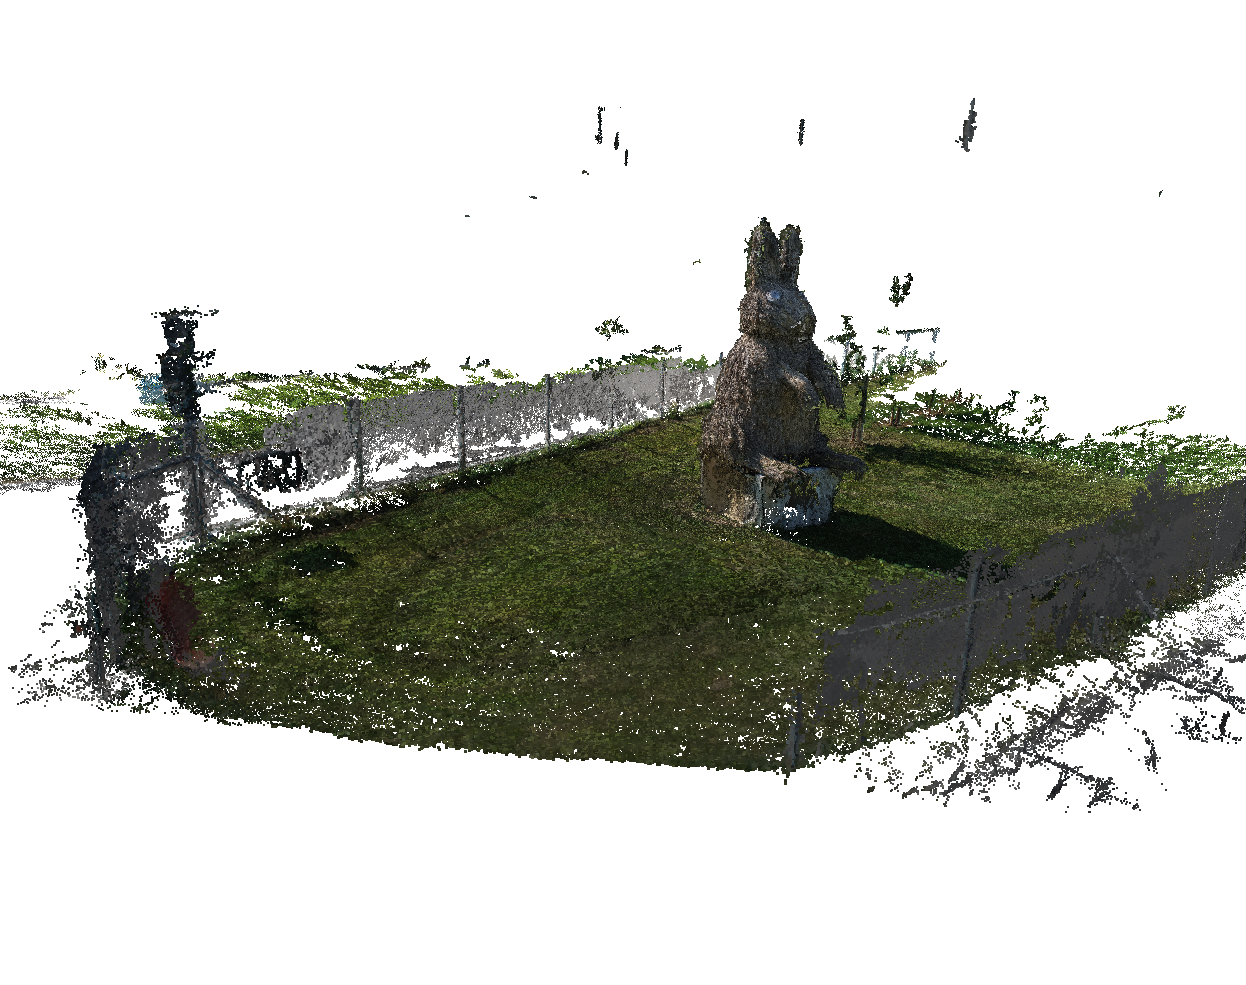
\includegraphics[width=20cm,angle=90]{images/rabbit-dense-vsfm.png}
	}
	\caption{Resultat: Punktwolke Hase mit VSFM}
	\label{img:rabbit-dense-vsfm}
\end{figure}

\begin{figure}[p]
	\centerline{
		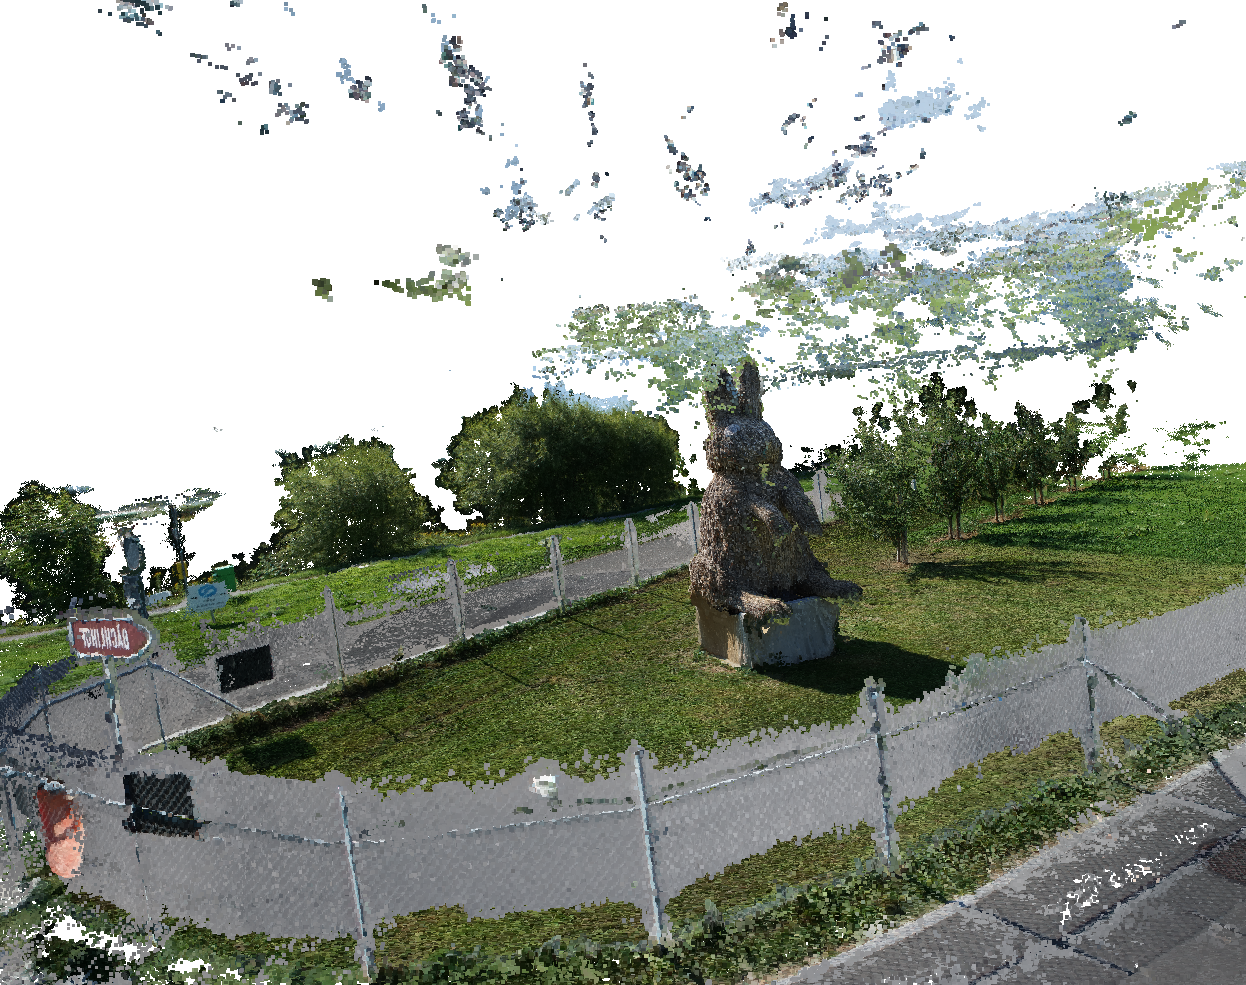
\includegraphics[width=20cm,angle=90]{images/rabbit-dense-pix4d.png}
	}
	\caption{Resultat: Punktwolke Hase mit Pix4DMapper Pro}
	\label{img:rabbit-dense-pix4d}
\end{figure}

\begin{figure}[p]
	\centerline{
		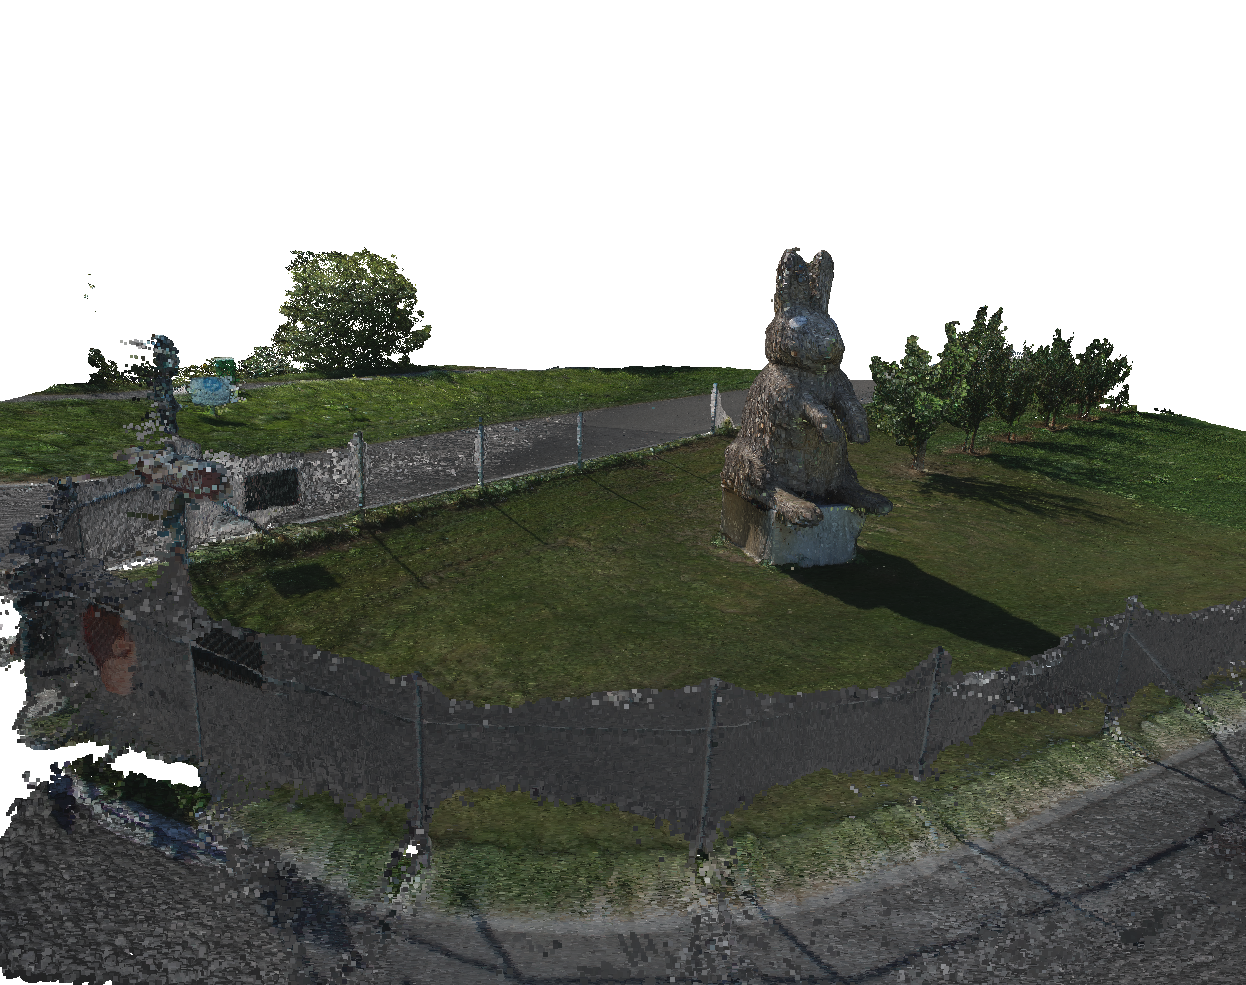
\includegraphics[width=20cm,angle=90]{images/rabbit-dense-photoscan.png}
	}
	\caption{Resultat: Punktwolke Hase mit PhotoScan Pro}
	\label{img:rabbit-dense-photoscan}
\end{figure}

%----------------------------------------------------------------------------------------

\begin{figure}[p]
	\centerline{
		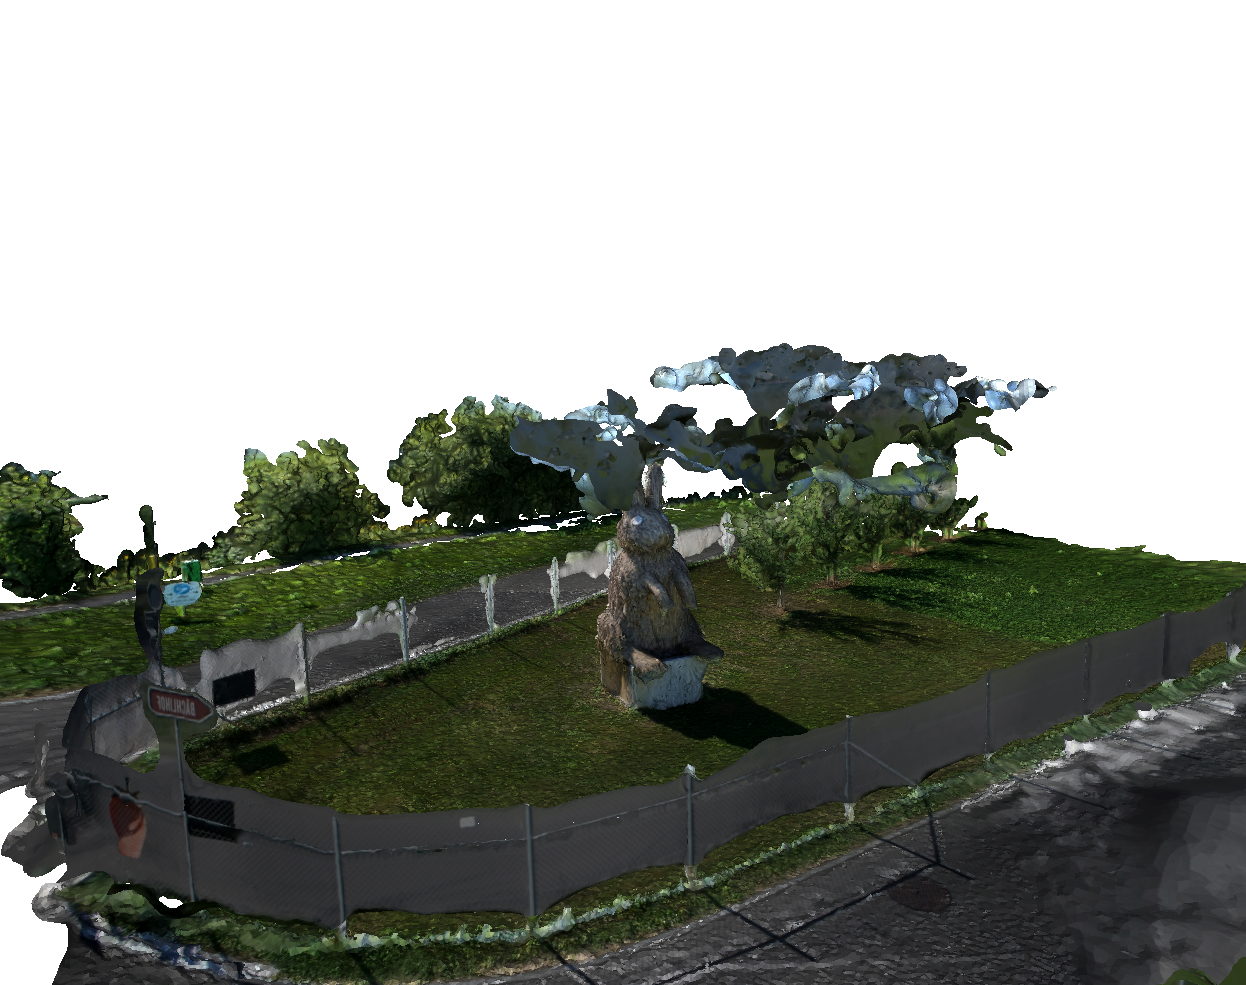
\includegraphics[width=20cm,angle=90]{images/rabbit-mesh-pix4d.png}
	}
	\caption{Resultat: Mesh Hase mit Pix4DMapper Pro}
	\label{img:rabbit-mesh-pix4d}
\end{figure}

\begin{figure}[p]
	\centerline{
		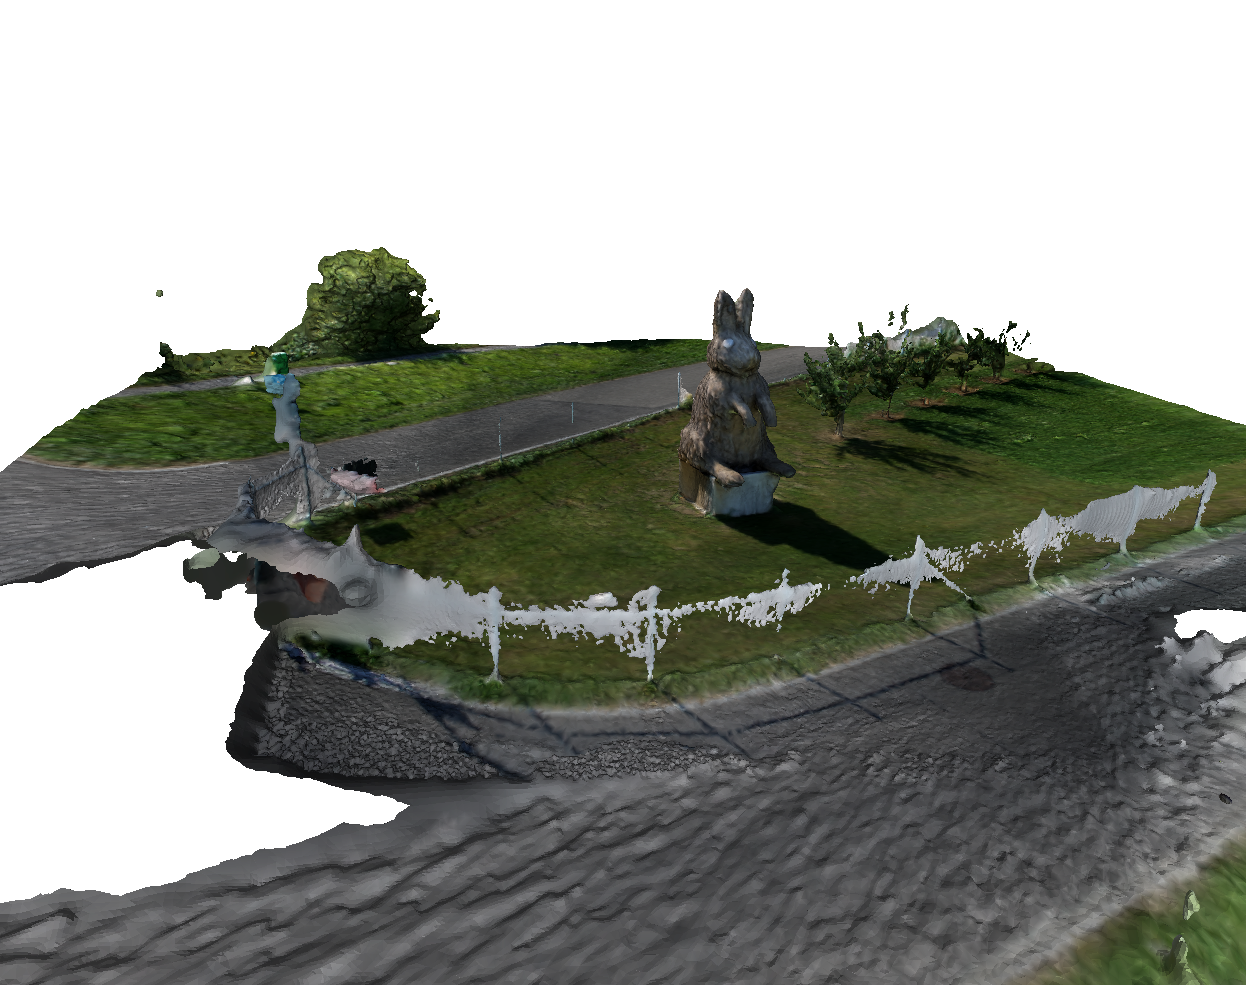
\includegraphics[width=20cm,angle=90]{images/rabbit-mesh-photoscan.png}
	}
	\caption{Resultat: Mesh Hase mit PhotoScan Pro}
	\label{img:rabbit-mesh-photoscan}
\end{figure}

%----------------------------------------------------------------------------------------
